\chapter{Vaatimustenkeruusuunnitelma} % Itse luvun otsikko. Huom ei numeroa!
\label{keruu} % Tähän kappaleeseen voi viitata \ref{keruu}
\thispagestyle{fancy} % Tarvitaan, jotta header/footer näkyvät otsikkosivuilla

Tässä luvussa käsitellään jo olemassa olevia dokumentaatioita, ja mitä vaatimuksia asiakastietojärjestelmälle voidaan niiden perusteella määrittää. Luvussa esitellään erilaisia tapoja, joita voidaan hyödyntää vaatimusten keruussa sidosryhmiltä.\cite{kurssi}

\section{Taustatilanne}

Megantti konsernilla ei ennestään ollut käytössä keskitettyä asiakkuudenhallintajärjestelmää (\acrshort{crm}) \cite{crm}.
Asiakastietoja ovat keränneet lähinnä myyntipuolen työntekijät, joilla on ollut ongelmia tietojen jakamisessa keskenään sekä asiakastietojen tietosuojaan liittyen. Uuden CRM:n olisi tarkoitus keskittää tietojen hallinnointi ja tasapuolistaa erityisesti eri myyntihenkilöiden informatiivista asemaa asiakkaita kohtaan.

\section{Nykyisen dokumentaation analyysi}
Tässä kappaleessa analysoidaan olemassa olevaa dokumentaatiota. Tämän analyysin pohjalta määritetään alustavia vaatimuksia.


    \subsection{Kehyskertomuksen analyysi}
    Con-Salting Oy on luonut järjestelmälle kehyskertomuksen \cite{kurssi}. Siinä määritetään asiakastietojärjestelmälle alustavia vaatimuksia. Kehyskertomuksen perusteella voidaan määrittää sidosryhmiä, jotka tulee ottaa huomioon, ja joiden kanssa tulee kommunikoida vaatimuksia määriteltäessä.

    Tällaisia sidosryhmiä ovat muun muassa yrityksen johto ja myynti- ja markkinointiosasto.
    Sidosryhmät ovat esittäneet toivomuksina esimerkiksi asiakastietojärjestelmän nopean toiminnan, käytettävyyden erilaisilta päätelaitteilta sekä asiakkaan 
    automaattisen profiloinnin. 
        
    Kehyskertomuksessa ilmenee myös muita asioita jotka tulee ottaa huomioon:
    
    \begin{itemize}
        \item Järjestelmän tulee olla yhteensopiva muiden yrityksen järjestelmien kanssa, kuten yrityksen varastojärjestelmän kanssa.
	    \item Asiakastietojärjestelmän tulee myös olla \gls{gdpr} mukainen
        \item Järjestelmän tulee pystyä hoitamaan joitain asioita automaattisesti, kuten suurostobonukset.
    \end{itemize}

    Nämä vaatimukset ovat kuitenkin ainoastaan suuntaa antavia, ja niitä tulee tarkentaa vaatimustenkeruussa. 


\section{Vaatimustenkeruumetodit}

    Vaatimustenkartutusmetodit voidaan jakaa kahteen eri osa-alueeseen: Epäsuoriin- ja suoriin metodeihin.
    Tässä kappaleessa käsitellään Megantin asiakas\-tietojärjes\-tel\-män kehitystä varten käytettäviä metodeja.


    \section*{Suorat metodit}

        Suorissa kartutustekniikoissa järjestelmän vaatimuksia kartoitetaan yhdessä sidosryhmien kansssa.
        Seuraavia suorakartutustekniikoita hyödynnetään mahdollisimman kattavan analyysin toteuttamiseen:

        \subsubsection*{Haastattelut}

            Sidosryhmille järjestetään kahdentyyppisiä haastatteluja. Ensimmäisessä haastattelussa haastateltavat vastaavaat ennalt\-amääriteltyihin kysymyksiin. 
            Ensimmäisten kysymysten tarkoituksena on luoda selkeä kuva nykytilanteesta ja sen mahdollisista ongelmakohdista. Toisessa haastattelussa haastattelu toteutetaan avoimesti. Haastateltaville esitetään erilaisia kysymyksiä järjestelmän toiminnalisuuteen liittyen, jolloin haastateltavien kanssa voidaan vuorovaikutteisesti pohtia millainen järjestelmän tulisi olla.

        \subsubsection*{Havainnointi}

            Meganttiin lähetetään 2 kehitys\-tiimiläi\-stä tark\-kailemaan mitkä ovat nykyisen jär\-jes\-telmän hyvät ja huonot puolet. Nämä tiimiläiset seuraavat noin kahden viikon ajan Megantin työn\-teki\-jöiden työtä ja tekevät 
            muistiinpanoja työntekijöiden tarpeista järjestelmään liittyen. He havainnoivat myös mitä puutteita ja vahvuuksia nykyisessä asiakastietojärjestelmässä on ja raportoivat näistä suoraan prototyyppien kehitystiimille. Havainnointi tiedonkeruumenetelmänä on tärkeää, sillä ihmisten on usein vaikea pukea arkipäivän työntekoa sanoiksi. Havainnoinnin avulla pystytään rakentamaan järjestelmä, joka vastaa myös tosielämän tarpeita.


        \subsubsection*{Ryhmätapaamiset}

            Projektin aikana järjestetään tapaamisia sidosryhmien kanssa. Näissä tapaamisissa kehitystiimi on suoraan kontaktissa kyseisen ryhmän kanssa ja ryhmän on mahdollista kertoa asiakastietojärjestelmän nykytilasta, kuvailla tilanteita ja havainnollistaa kuinka he haluaisivat järjestelmän toimivan kyseisissä tilanteissa.


    \section*{Epäsuorat metodit}

        Epäsuorissa kartutustekniikoissa sidosryhmiin ei olla suorassa kontaktissa, vaan käytetään jo ennalta olemassa olevia tietoja.
        Epäsuoraan kartutukseen käytetään seuraavia tekniikoita:

        \subsubsection*{Taustatutkimus}

        Con-Salting Oy on kerännyt jo muutamia yrityksen vaatimuksia kehyskertomukseen. 
        Näitä vaatimuksia ovat esimerkiksi asiakastietojen ylläpito ja asiakkaiden profilointi.
        Vaatimukset ovat kuitenkin löysästi määriteltyjä ja vaativat tarkennusta.

	Kartoittaa tulee ainakin nykyiset käytössä olevat järjestelmät (tietokannat, ohjelmistot jne), jotta saadaan tietoon, mitä vanhoja järjestelmiä voidaan suoraan korvata uudella ja mitkä vanhat järjestelmät ovat tuotannon kannalta välttämättömiä. Tämä kartoitus on tärkeää tehdä, jotta tiedetään, millaisten järjestelmien kanssa uuden järjestelmän tulee olla yhteensopiva.

        \subsubsection{Kyselyt}

        Osalle järjestelmän sidosryhmistä järjestetään kyselyitä, jossa selvitetään heidän mielestään tärkeimpiä järjestelmän vaatimuksia.
        Tällaisia sidosryhmiä ovat sisäiset käyttäjät, kuten yrityksen johto-, asiakaspalvelu- ja järjestelmän ylläpitohenkilöstö.

        \subsubsection*{Prototyypit}

        Sisäisille käyttäjille valmistetaan kahteen otteeseen prototyyppi järjestelmästä. Ensimmäisen vaiheen prototyypin on tarkoitus varmistaa yhteensopivuus vanhojen järjestelmien kanssa ja varmistaa ettei olennaisia komponentteja puutu valmiista järjestelmästä. Toisen vaiheen prototyyppi keskittyy ominaisuuksien hiomiseen ja tässä vaiheessa kehitystä ohjaavat vahvasti erinäiset ryhmätapaamiset ja haastattelut käyttäjien kanssa.
	
\section{Sidosryhmäanalyysi}

        Kuvassa \ref{img:sidosryhmat} (sivulla \pageref{img:sidosryhmat}) on esitelty erilaisia ohjelmistoon liittyviä sidosryhmiä ajatuskartan muodossa. \cite{kurssi}

        \begin{figure}[H] % tämä H tarkoittaa tekstin mukana { h | t | b | p | H}
		\centering
		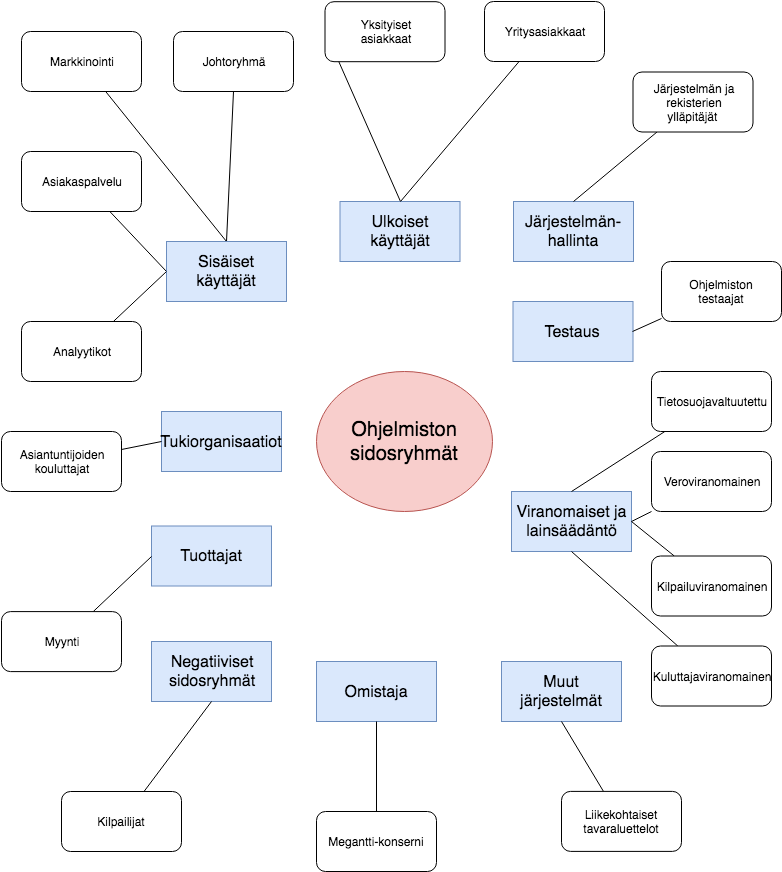
\includegraphics[width=\textwidth]{sidosryhmat.png}
		\caption{Ohjelmiston sidosryhmät} % Raportissa tulee olla selite jokaisen kuvan/kuvion/taulukon alla
		\label{img:sidosryhmat}
	\end{figure}

	Taulukkoon \ref{tab:sidosryhmataulukko} on kerätty tietoja sidosrymistä ja niiden suhteista.

\section{Alustavat havaitut vaatimukset ja luokittelu}
Taulukossa \ref{tab:sidosryhmataulukko} on havainnollistettu alustavia vaatimuksia. Taulukossa on myös määritelty vaatimusten keskinäisiä tärkeysjärjestyksiä.

    
\section{Vaatimusten keruuprojektin aikataulu}

	Vaatimusten keruun aikatulua on havainnollistettu Gantt-taulukon muodossa (Liitteessä \ref{aikatauluesimerkki}). Taulukosta ilmenee mikä vaatimusten keruumenetelmä on käytössä milloinkin.

